% SLIDE GENERATION INSTRUCTIONS

% For each slide I will paste in latex code with comments.
% For each comment, identify how to best address it
% considering the other comments and the context from the paper.

% To address each comment, ONLY write the changes you propose
% in code blocks I can easily paste into the latex document.
% For each code block explain HOW your changes address my comments.
% Think step-by-step and always identify your previous issues first.
% Make sure to output latex that is at most 80 chars per line,
% make plenty line breaks to ensure good readability.

% When writing slides, please make sure to keep this logical
% structure so that it is still understandable.
% It must have a narrative, that is very important.
% Split one 'slide' into multiple pages using the package and
% \only<slide number, e.g. 1, 2 or even '1-2' for both> {..} to make it more easy to follow
% for listeners.

% Your output should look like this:
% ## Slide <num>: <slide title>
% This slide addresses the comment <comment from latex> by
% <one sentence explanation of slide contents>.
% ```latex
% \only<1> { % Slide 1 content, narrative, etc. }
% \only<2-3> { % Slide 2, transition to 3 }
% \only<3> { % Slide 3 content, narrative, etc. }
% ```

\documentclass{beamer}
\usetheme{Madrid} 
\usepackage{graphicx}
\usepackage{hyperref}
\usepackage{tikz}
\usepackage{pgfplots}
\usetikzlibrary{positioning}

\title{Nonsmooth Optimization via Quasi-Newton Methods}
\author{Adrian S. Lewis and Michael L. Overton}
\date{}

\begin{document}

\begin{frame}
    \titlepage
\end{frame}

\begin{frame}{Outline}
    \tableofcontents
\end{frame}

\section{Introduction}
\begin{frame}{Basics of Optimization}
    % Slide 1: Define Optimization Problem
    % Slide 2: Write out Taylor Approximation
    % Slide 3: Explain Gradient Descent

    \only<1> {
        The general unconstrained optimization problem
        is given by:
        \begin{equation*}
            \min_{x \in \mathbb{R}^n} f(x),
        \end{equation*}
        where $f: \mathbb{R}^n \to \mathbb{R}$ is a
        twice-differentiable real-valued function.
    }

    \only<2-3> {
        % First-order Taylor approximation
        The first-order Taylor approximation
        of $f$ around $x_k$ yields:
        \begin{align*}
            f(x) & \approx f(x_k) + \nabla f(x_k)^T (x - x_k).
        \end{align*}
    }

    \only<3> {
        Which motivates the Gradient Descent method as follows:
        \begin{align*}
            x_{k+ 1} = x_k - t_k \nabla f(x_k),
        \end{align*}
        where $t_k > 0$ is some step size.
    }
\end{frame}

\begin{frame}{Newton's Method}
    \only<1-2> {
        % Second-order taylor approximation
        The second-order Taylor approximation of $f$ around $x_k$ yields:
        \begin{align*}
            f(x) & \approx f(x_k) + \nabla f(x_k)^T (x - x_k)           \\
                 & + \frac{1}{2} (x - x_k)^T \nabla^2 f(x_k) (x - x_k).
        \end{align*}
        A necessary condition for a local minimizer $x_k$
        is that $\nabla f(x_k) = \mathbf{0}$.
    }

    \only<2> {
        % Also from Taylor Approximation
        \vspace{0.5em}
        `Jumping' to the minimizer of this quadratic
        approximation yields Newton's Method:
        \begin{align*}
            x_{k+1} = x_k - (\nabla^2 f(x_k))^{-1} \nabla f(x_k),
        \end{align*}
        where $\nabla^2 f(x_k)$ is the Hessian matrix.
    }
\end{frame}

\section{Quasi-Newton Methods}
\begin{frame}{Quasi-Newton Methods}
    % Define QN method as in the paper
    \only<1> {
        The main disadvantage of Newton's method
        is the need to compute
        the Hessian matrix $\nabla^2 f(x_k) \in \mathbb{R}^{n \times n}$
        and solve a linear system of equations
        in every iteration.

        \vspace{0.5em}
        Also, the true Hessian might not always be positive definite.
    }

    \only<2> {
        Quasi-Newton methods approximate the
        \textbf{inverse} Hessian
        $$H_k \approx (\nabla^2 f(x_k))^{-1}$$
        by iteratively updating $H_k$.
    }

    \only<3> {
        \begin{block}{Algorithm 1 (quasi-Newton method)}
            Choose $x_0$ with $f$ differentiable at $x_0$,
            set $H_0$ to a positive definite matrix and
            $k \leftarrow 0$

            \texttt{repeat}

            \qquad compute search direction $p_k \leftarrow -H_k \nabla f_k$

            \qquad set $x_{k + 1} \leftarrow x_k + t_k p_k$,
            where $t_k > 0$ \\
            \qquad\qquad is chosen by a line search

            \qquad \texttt{if} $f$ is not differentiable at $x_{k + 1}$,
            or $\nabla f_{k + 1} = 0$, \\
            \qquad\qquad stop.

            \qquad set $y_k \leftarrow \nabla f_{k + 1} - \nabla f_k$

            \qquad choose $H_{k + 1}$ to be a positive definite matrix
            satisfying \\
            \qquad\qquad the secant condition $H_{k + 1} y_k = t_k p_k$

            \qquad $k \leftarrow k + 1$

            \texttt{end (repeat)}
        \end{block}
    }

    \only<4> {
        The true Hessian has the property
        \begin{align*}
            \nabla^2 f(x_{k}) \underbrace{
                (x_{k + 1} - x_k)
            }_{t p_k} =
            \underbrace{
                \nabla f(x_{k + 1}) - \nabla f(x_k)
            }_{y_k},
        \end{align*}
        by the Taylor expansion of $\nabla f$ at $x_k$,
        which results in the secant equation since
        $H_{k + 1} \approx (\nabla^2 f(x_k))^{\mathbf{-1}}$.
    }

    % Clarify a number of things from the algorithm
    \only<5> {
        The BFGS algorithm updates the inverse Hessian using:
        \begin{align*}
            H_{k + 1} & = V_k H_k V_k^T + t_k \frac{
                p_k p_k^T
            }{p_k^T p_k}                                   \\
            V_k       & = I - \frac{p_k y_k^T}{p_k^T y_k}.
        \end{align*}
    }
\end{frame}

\begin{frame}{Non-smooth Optimization}
    % Illustrate Problem of GD in non-smooth optimization, e.g. Abs value
    \only<1> {
        \begin{figure}
            % Abs value plot
            \begin{figure}
                \centering
                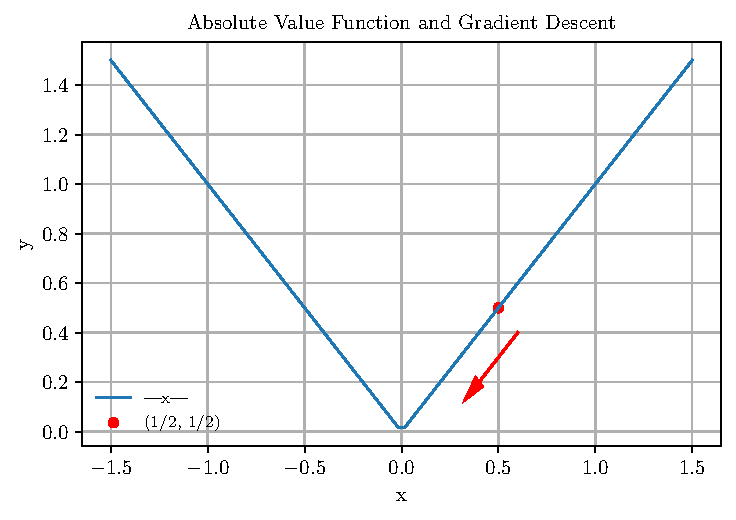
\includegraphics[width=0.7\textwidth]{plots/abs_val_func.pdf}
                \caption{The absolute value function and Gradient Descent
                    with $x_0 = \frac{1}{2}$ and $t_k = 1$.}
                \label{fig:abs_value_function}
            \end{figure}
        \end{figure}
    }

    \only<2> {
        The problem is that the gradient does not smoothly change
        near the minimum, but jumps from $-1$ to $1$.
        The gradient is not continuous at the minimum.
    }

    \only<3> {
        In fact, with \textbf{any constant step size} $t_k$,
        Gradient Descent will oscillate forever on this problem.
    }
\end{frame}

\section{Numerical Experiments}
\begin{frame}{Optimization Example on Euclidean Norm Function}
    \only<1> {
        % Euclidean norm plot
        \begin{figure}
            \centering
            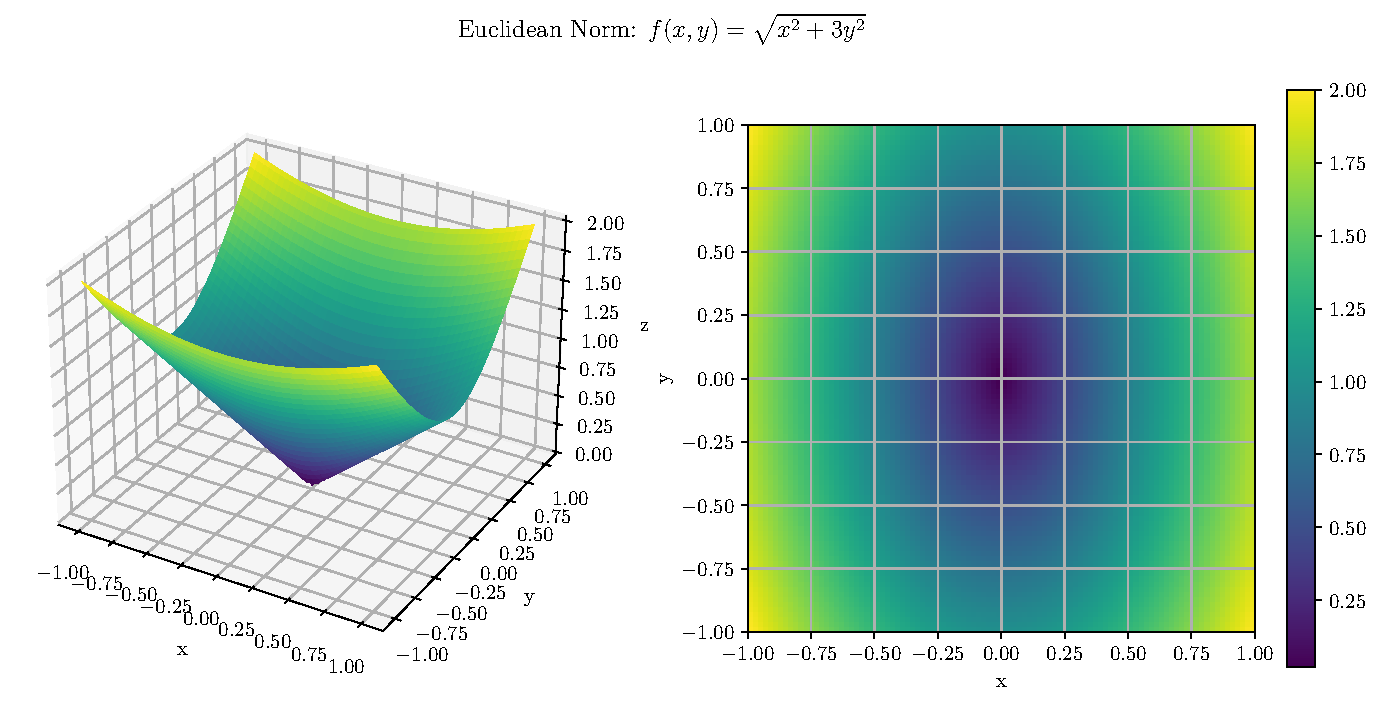
\includegraphics[width=1.0\textwidth]{plots/euclidean_norm.pdf}
            \caption{The (skewed) Euclidean norm function}
            \label{fig:euclidean_norm_function}
        \end{figure}
    }
    \only<2> {
        % Standard GD
        \begin{figure}
            \centering
            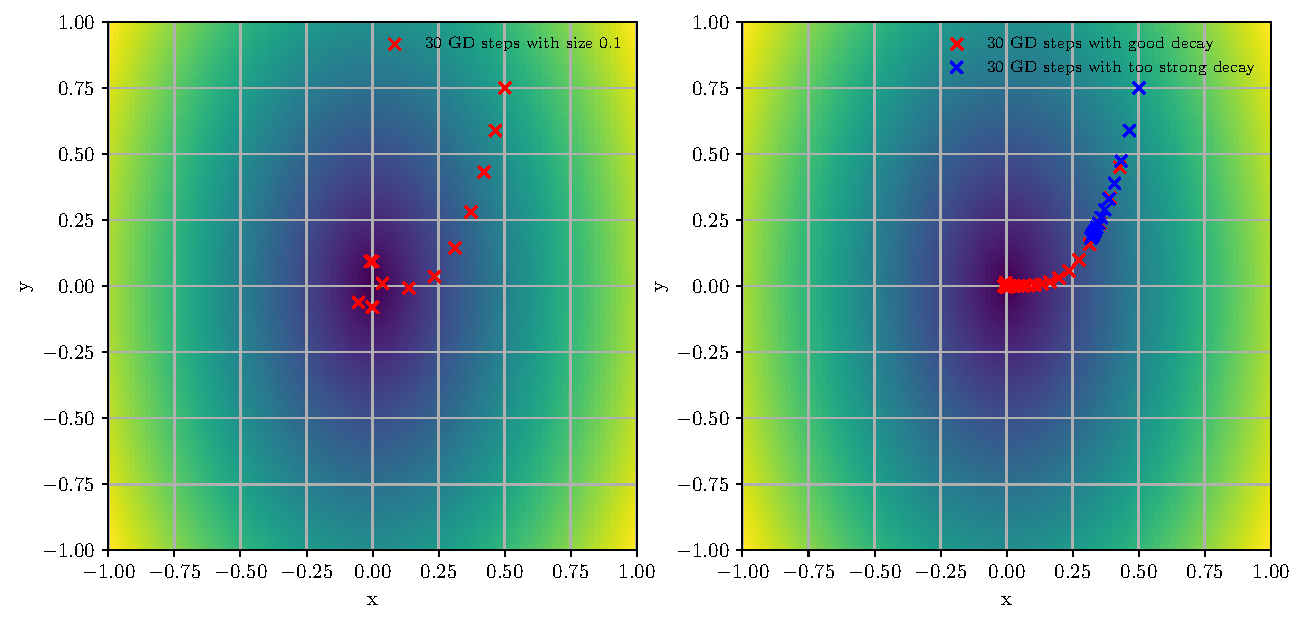
\includegraphics[width=1.0\textwidth]{plots/gd_steps.pdf}
            \caption{Gradient Descent with and without
                step size decay}
            \label{fig:gd_steps}
        \end{figure}
    }
    \only<3> {
        % GD & Newton with line search
        \begin{figure}
            \centering
            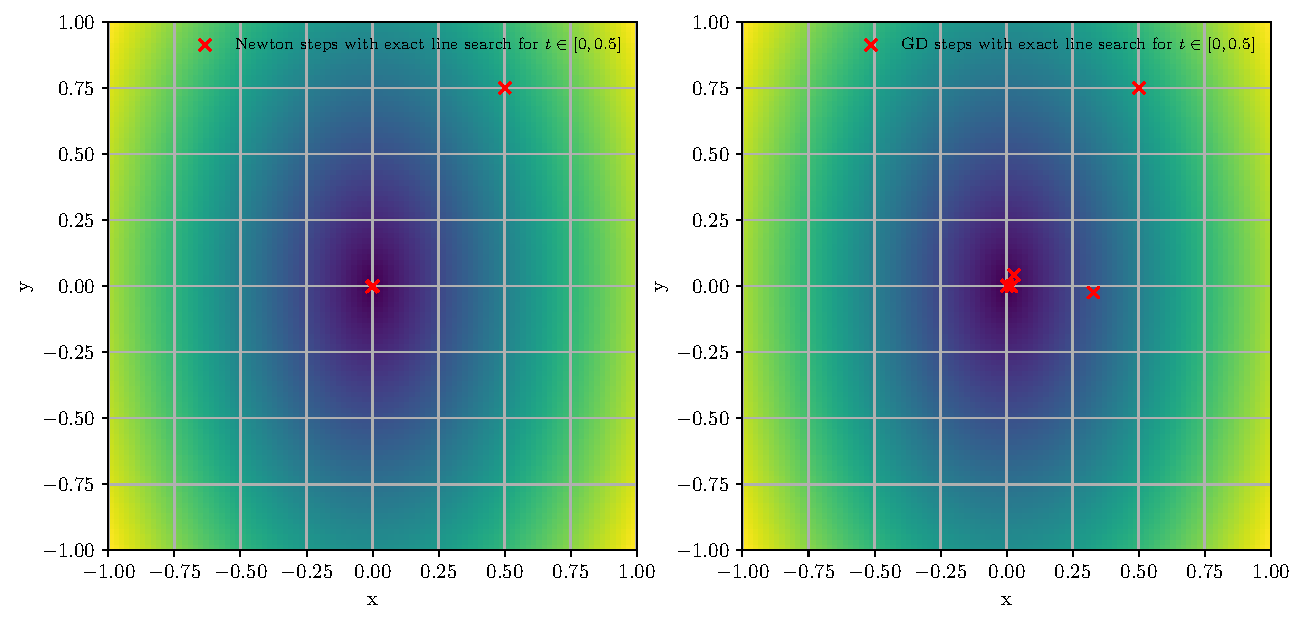
\includegraphics[width=1.0\textwidth]{plots/exact_line_search_newton_vs_gd.pdf}
            \caption{Newton and Gradient Descent
                with exact line search}
            \label{fig:newton_gd_exact_line_search}
        \end{figure}
    }
    \only<4> {
        % Newton Gradient Surface
        \begin{figure}
            \centering
            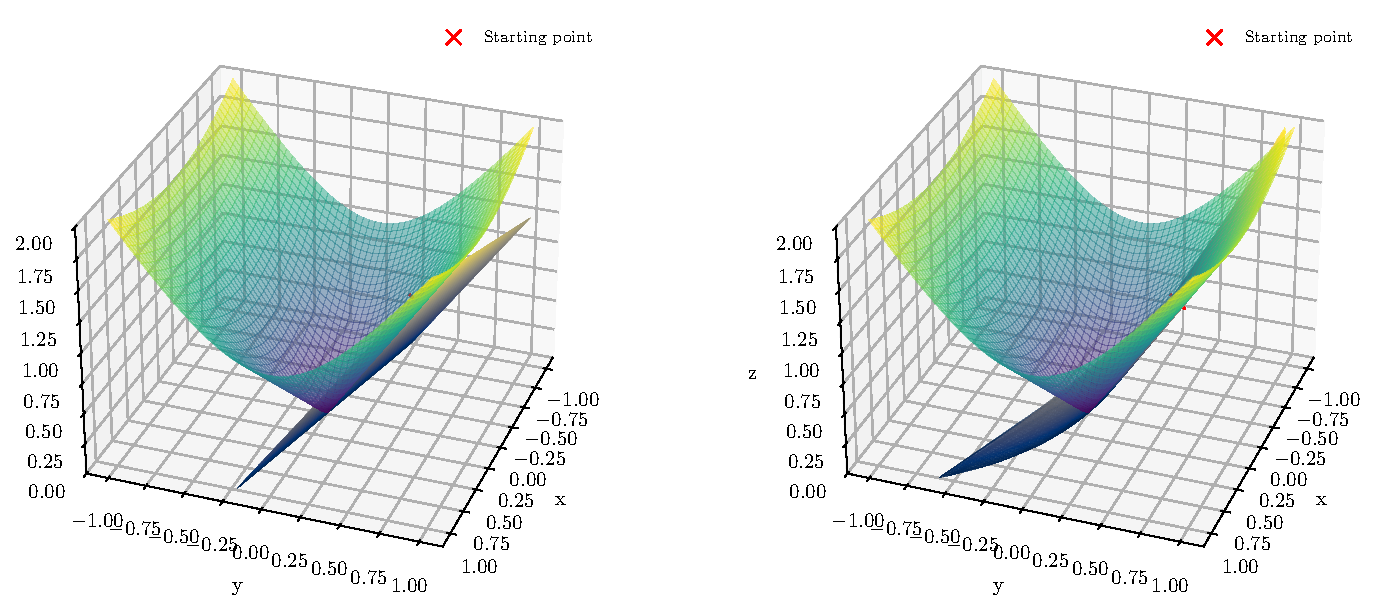
\includegraphics[width=1.0\textwidth]{plots/3d_newton_and_gradient_surface.pdf}
            \caption{First and second order Taylor approximations
                of $f$}
            \label{fig:3d_newton_gradient_surface}
        \end{figure}
    }
    \only<5> {
        % Newton Gradient Contour Plot
        \begin{figure}
            \centering
            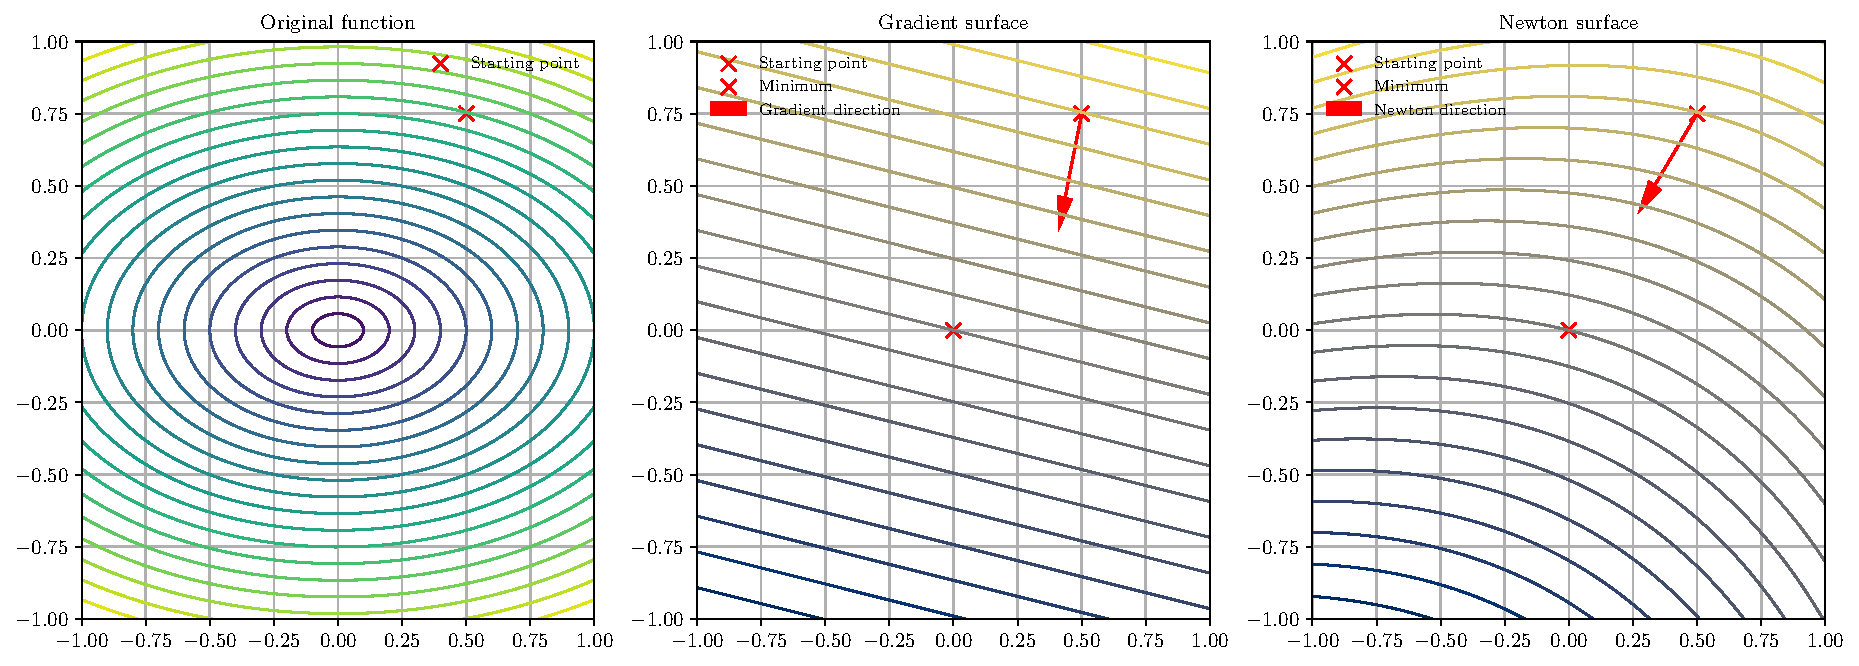
\includegraphics[width=1.0\textwidth]{plots/contour_newton_and_gradient_surface.pdf}
            \caption{Contour plot of the first and second order
                Taylor approximations of $f$}
            \label{fig:contour_newton_gradient_surface}
        \end{figure}
    }
\end{frame}

\subsection{Line Search}
\begin{frame}{Exact Line Search}
    % Define exact line search
    Given a search direction $p_k$ and a starting point $x_k$,
    \textbf{exact line search} solves:
    \begin{align*}
        t_k = \arg \min_{t > 0} f(x_k + t p_k).
    \end{align*}
    \\

    \only<2> {
        \vspace{0.5em}
        In (quasi-)Newton methods, we search $t \in [0, 1]$
        since we don't want to take steps larger
        than true newton would.
    }
    \only<3> {
        In non-smooth problems, exact line search could
        find an $x_{k + 1}$ where $f$ is not differentiable
        that \textbf{is not a minimizer}.
        \\
        \vspace{0.5em}

        E.g. for $f(x, y) = |x| + |y|$ and $x_k = (1, 0)$,
    }
\end{frame}

\begin{frame}{Armijo-Wolfe Conditions}
    % Define Armijo-Wolfe Conditions
    \only<1> {
        The \textbf{Armijo condition} ensures that
        the step size $t_k$ decreases the objective function
        sufficiently:
        \begin{align*}
            f(x_k + t_k p_k) \le f(x_k) + c_1 t_k \nabla f(x_k)^T p_k,
        \end{align*}
        where $0 < c_1 < 1$ is a constant.
    }
    \only<2> {
        \begin{figure}
            \centering
            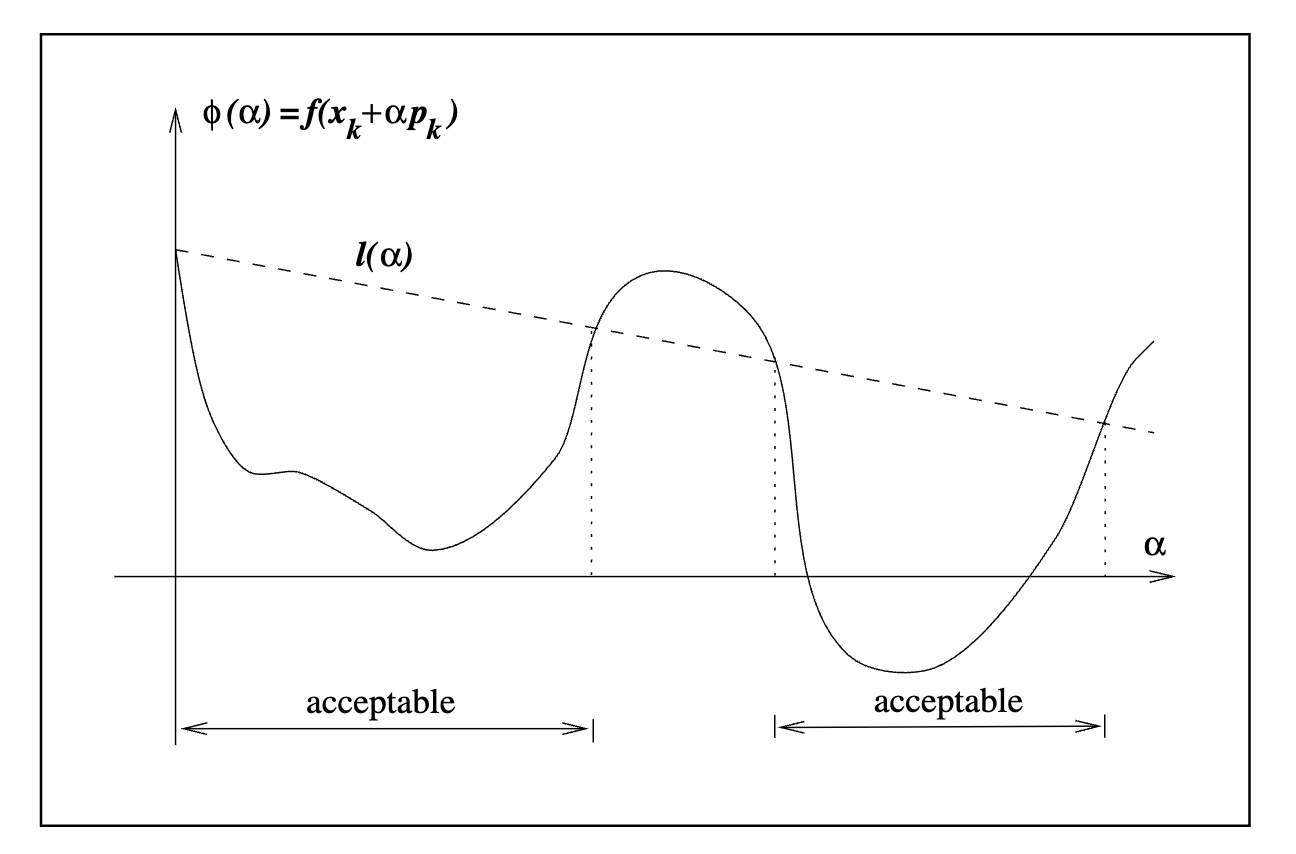
\includegraphics[width=0.7\textwidth]{plots/armijo_condition.png}
            \caption{Armijo condition ensuring sufficient decrease;
                Source: Numerical Optimization by Nocedal and Wright,
                Figure 3.3
            }
            \label{fig:armijo_condition}
        \end{figure}
    }
    \only<3> {
        However, the Armijo condition works for any sufficiently
        small step size $t_k$.
    }
    \only<4> {
        The \textbf{Wolfe condition} ensures that
        the step size $t_k$ is not too small:
        \begin{align*}
            \underbrace{
            \frac{\partial}{\partial t_k} (
            f(x_k + t_k p_k)
            )
            }_{
            \text{Slope of the LS objective}
            }
            =
            \nabla f(x_k + t_k p_k)^T p_k \ge c_2 \nabla f(x_k)^T p_k,
        \end{align*}
        where $c_1 < c_2 < 1$ is a constant.
    }

    \only<5> {
        The intuition here is that:
        if line search would still improve the objective,
        then we should keep going
    }

    \only<6> {
        \begin{figure}
            \centering
            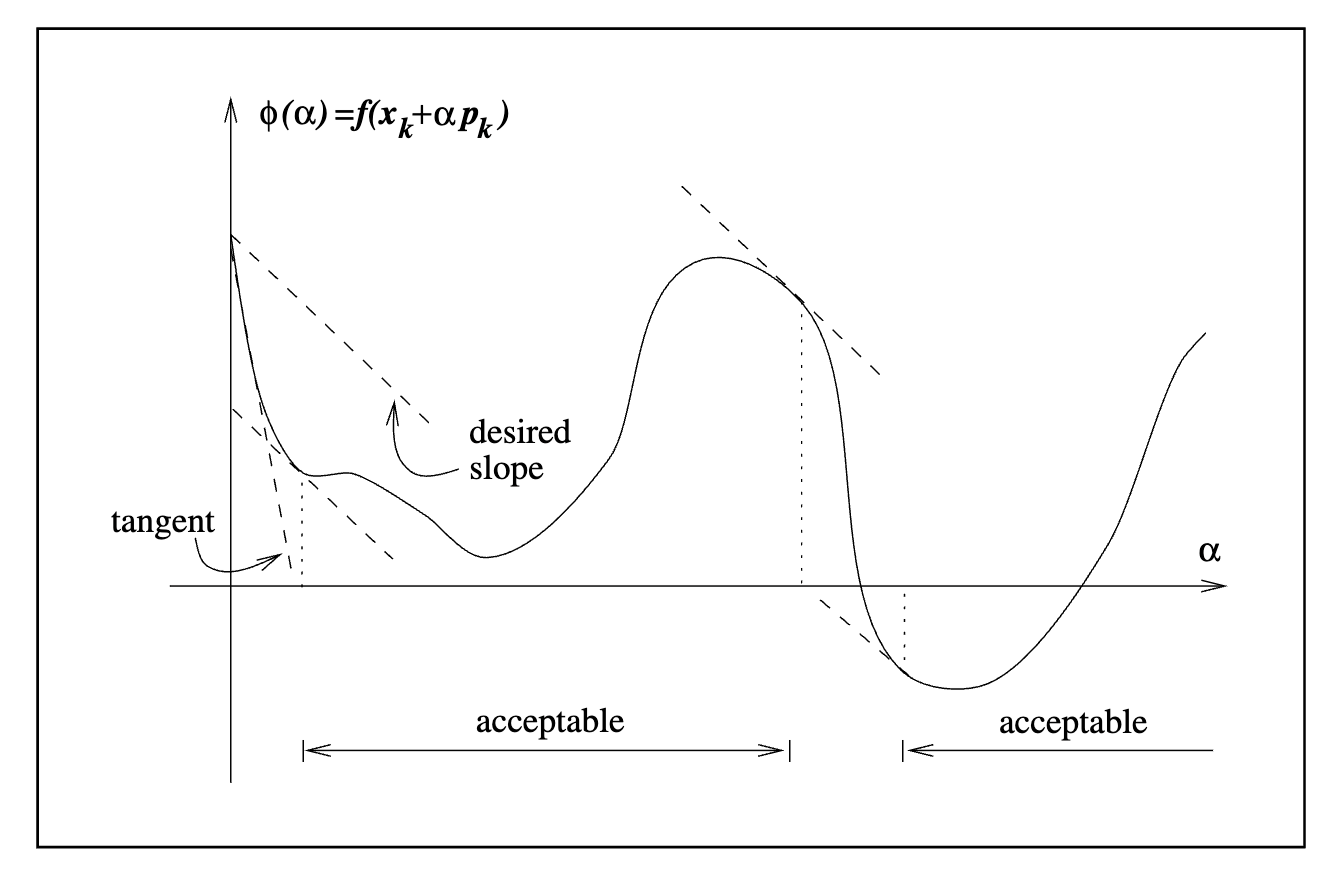
\includegraphics[width=0.8\textwidth]{plots/wolfe_condition.png}
            \caption{The Wolfe/Curvature condition;
                Source: Numerical Optimization by Nocedal and Wright,
                Figure 3.4}
            \label{fig:wolfe_condition}
        \end{figure}
    }
\end{frame}

\begin{frame}{Inexact Line Search}
    % Define Armijo-Wolfe Conditions
    \only<1-2> {
        Using these conditions,
        we can define an \textbf{inexact line search}:
        \begin{block}{Algorithm 2 (inexact line search)}
            $\alpha \gets 0 \qquad \beta \gets +\infty \qquad t \gets 1$

            \textbf{repeat}

            $\quad \textbf{if } A(t) \textbf{ fails } \beta \gets t$

            $\quad \textbf{elseif } W(t) \textbf{ fails } \alpha \gets t$

            $\quad \textbf{else  stop}$

            $\quad \textbf{if } \beta < +\infty \quad t \gets (\alpha + \beta)/2$

            $\quad \textbf{else }  t \gets 2\alpha$

            \textbf{end(repeat)}
        \end{block}
    }
    \only<2> {
        Here, the Wolfe condition $W(t)$ implicitly
        checks differentiability of $f$ at $x_k + t p_k$.
    }
    \only<3> {
        Inexact line search is great because we can apply
        quasi-Newton methods to non-smooth problems.
    }
\end{frame}

\section{Conclusion}
\begin{frame}{Conclusion}
    In Summary:
    \begin{itemize}
        \item (quasi-)Newton gives us the best search direction
              and hence faster convergence,
              but comes at additional $n^2$ cost for the Hessian.
        \item With inexact line search, this works well
              for non-smooth problems where exact line search
              can fail
        \item If function evaluation and gradient computation
              are cheap, Gradient Descent is likely the best choice,
              but line search is always crucial!
    \end{itemize}
\end{frame}

\begin{frame}{Conclusion}
    \begin{center}
        Thank you for your attention!
    \end{center}
\end{frame}

\end{document}